\documentclass[conference]{IEEEtran}
\usepackage[T1]{fontenc}
\usepackage{amsmath}
\usepackage{booktabs}
\usepackage{array}
\usepackage{graphicx}
\usepackage{multirow}
\usepackage{balance}
\usepackage{url}
\usepackage{xcolor}
\usepackage[hidelinks]{hyperref}
\newcommand{\toverify}{\textcolor{red}{[TO VERIFY]}}
\newcommand{\verifyitem}[1]{\textcolor{red}{[TO VERIFY: #1]}}

\title{A Source-Guided Reproduction of BioBERT for Four-Class Causal-Language Classification}
\author{\IEEEauthorblockN{Anand Kumar}\\\IEEEauthorblockA{Indian Institute of Information Technology Allahabad , Prayagraj}\\\IEEEauthorblockA{rsi2026511@iiita.ac.in}}
\begin{document}
\maketitle

% ABSTRACT IS PLACED FIRST AS REQUIRED BY IEEEtran, BUT WRITTEN LAST
% FROM THE EVIDENCE PRESENTED IN THE BODY.
\begin{abstract}
We report a source-guided modern reproduction of a published four-class BioBERT causal-language classification baseline on 3,061 PubMed sentences. Five-fold stratified cross-validation yielded mean held-out accuracy of 0.8981 (sample standard deviation 0.0076) and mean macro-F1 of 0.8822 (sample standard deviation 0.0075), compared with published rounded values of 0.900 and 0.883, respectively. Independent audits verified all 3,061 out-of-fold prediction assignments, gold-label alignment, probability normalization, and agreement between saved predictions and reported metrics. Restored checkpoints reproduced all held-out labels for four folds and eight labels for the remaining fold. The numerical agreement is close, but historical fold identities, original pretrained-checkpoint equivalence, and exact optimizer equivalence remain unverified. These results establish an auditable modern classification baseline, but no controlled extension or paired editing evaluation has yet been executed; no causal-meaning preservation claim is made.
\end{abstract}

\begin{IEEEkeywords}
BioBERT, causal language, correlational language, baseline reproduction, stratified cross-validation, reproducibility
\end{IEEEkeywords}

\section{Introduction}\label{sec:intro}
Distinguishing causal claims from correlational statements is important when interpreting scientific language. A four-class sentence classification benchmark is one way to evaluate a system's ability to distinguish statements describing no relationship, direct causality, conditional causality, and correlation. The published source repository reports five-fold mean accuracy of 0.900 and macro-F1 of 0.883 for the study by Yu et al.~\cite{yu2019detecting}. These are rounded source-reported benchmarks, not paired measurements on our fold assignments.

Our immediate aim is narrower than demonstrating faithful editing by a large language model: we examine whether the published classification baseline can be reproduced in a documented contemporary environment while preserving its central architecture and optimization choices. The contribution of this work is an auditable implementation-and-evaluation record: immutable fold-index manifests, held-out prediction files, independently recomputed metrics, and checkpoint-restoration tests. We do not introduce a new causal-classification architecture or claim that predicted label agreement measures semantic equivalence of edited text.

We investigate three empirical questions. First, how closely do five-fold results approach the published rounded reference values? Second, how does performance differ across classes and folds? Third, which aspects of methodological equivalence remain uncertain despite numerical agreement? A separate research question---whether language-model edits preserve causal semantics---is explicitly outside the tested scope because no edited sentence pairs were evaluated.

\section{Related Work}\label{sec:related}
\subsection{Published causal-language baseline}
The original study by Yu, Li and Wang~\cite{yu2019detecting} and its released implementation provide the methodological point of comparison. The authoritative ACL Anthology lists pages 4664--4674, unlike the pages 4656--4666 printed in the source repository README; the former are used in our BibTeX record. The inspected released script applies five-fold stratified cross-validation, BioBERT-based four-class classification, five training epochs, and class-weighted learning. These are previously published choices, not methods newly proposed in this reproduction.

\subsection{Biomedical pretrained language models}
The reproduced classifier uses a biomedical BERT encoder, identified in the modern environment as \texttt{dmis-lab/biobert-base-cased-v1.1}. BioBERT was introduced by Lee et al.~\cite{lee2020biobert} as biomedical-domain language-model pretraining. The model family predates the reproduction; its biomedical pretraining is not our contribution. The original historical archive and Hugging Face checkpoint have not been compared tensor by tensor.

\subsection{Language-preserving editing}
The broader motivation concerns preserving causal and correlational meaning when scientific statements are edited. However, the evaluated corpus consists of individually labeled sentences rather than independently annotated source--edited sentence pairs. We therefore make no comparative claim against causal-preservation benchmarks or editing systems, and add no unverified citations. The user-supplied prior literature review proposes edit-pair evaluation and counterfactual semantic tests; such experiments are future work rather than measured outcomes in this study. A comprehensive current novelty search and the review's nonprimary bibliographic metadata remain [TO VERIFY].


\section{Research Questions and Evidence Boundaries}\label{sec:rq}
The research motivation originates in an earlier review on causal versus correlational language in LLM-assisted editing. That review proposes an edit-pair benchmark with annotated causal inflation, attenuation, hedge deletion and reversal of direction. This paper focuses deliberately on the prerequisite sentence-label classifier because no genuine, expert-annotated source--edit pair dataset or model-generated edited sentences were evaluated. Consequently, we study the following reproducibility-focused questions rather than claiming editing preservation.

\emph{RQ1 (numerical reproduction):} Under a documented modern software environment, how closely does a source-guided implementation approach the released benchmark's rounded five-fold metrics? The primary outputs are fold-mean accuracy and macro-F1; they do not directly identify an optimizer or pretraining effect. \emph{RQ2 (error characteristics):} What class-specific errors can be derived from nonoverlapping out-of-fold predictions? We examine the pooled confusion matrix and class-specific precision/recall. \emph{RQ3 (traceability):} Do the saved prediction and checkpoint artifacts support the reported evaluation? We assess original row IDs, labels, probability vectors, final-epoch selection, manifest hashes and reloaded checkpoints.

We do not test hypotheses of improvement over the original implementation, causal-direction understanding, inter-annotator reliability, domain transfer or LLM-editing fidelity. The associated unexecuted proposal is documented in the supplementary project brief. Although the assignment encourages two meaningful comparators where feasible, this completed baseline experiment does not include two independently executed classifiers; claims of comparative superiority are therefore excluded.

\section{Source-to-Implementation Verification}\label{sec:trace}
\begin{table}[t]
\centering
\caption{Historical Source Versus Modern Reproduction}\label{tab:trace}
\begin{tabular}{@{}p{0.22\columnwidth}p{0.31\columnwidth}p{0.35\columnwidth}@{}}
\toprule
Feature & Historical source & Modern reproduction\\
\midrule
Sentence cleaning & Whitespace strip; cased input & Same rule observed\\
Outer 5-fold split & Stratified; output sizes 614/613/613/611/610 & Stratified, saved sizes 613/612/612/612/612\\
Internal validation & 5\% via global RNG/random split & 5\% via separately seeded permutation\\
Architecture & BioBERT pooled output + dropout + 4-class head & Same structural form; modern checkpoint\\
Optimization & Historical BertAdam, per-tensor clipping, no bias correction & Source-guided equivalent in tested toy cases; exact historical run uncertain\\
Weighting & Whole-corpus balanced class weights & Whole-corpus weights, including held-out frequency information\\
Checkpoint selection & Last epoch after 5 epochs & Last epoch after 5 epochs\\
\bottomrule
\end{tabular}
\end{table}

The source-to-implementation comparison in Table~\ref{tab:trace} distinguishes a verified design match from a nonidentical execution environment. The repository inspected for the 2019 baseline was at commit \texttt{84abecc88b201a5ce27e1622597f780a9800c498}; a modified historical optimizer dependency was inspected at \texttt{5f63b4c3ec3f3c4c06a73713a57f7a5f9354ae10}. The independent architecture and optimizer sanity checks establish implementation behavior in selected cases, not an exhaustive semantic equivalence proof. Prior to any new experiment, the modern fold manifests were fixed, and no hyperparameters were changed based on held-out accuracy.

\section{Methodology}\label{sec:method}
\subsection{Dataset and labels}
We retained all 3,061 rows of the original PubMed causal-language CSV and used the four labels: 0, no relationship (1,356 rows); 1, direct causal (494); 2, conditional causal (213); and 3, correlational (998). Text was stripped of leading and trailing whitespace, without lowercasing, and encoded with the case-sensitive BioBERT tokenizer. The earlier data audit identified seven duplicate sentence pairs, including one pair with conflicting labels, and possible encoding artifacts in 32 rows. These were not silently removed or repaired.

\subsection{Partition protocol}
Five outer folds were generated with \texttt{StratifiedKFold(n\_splits=5, shuffle=True, random\_state=0)} in the contemporary environment. For each outer training portion, a 5\% internal validation subset was allocated using a separately seeded PyTorch permutation. The fit/validation/test sizes were 2,326/122/613 for fold 0 and 2,327/122/612 for folds 1--4. The outer test records were disjoint by row index and covered every corpus record exactly once. The historical implementation used a different internal random-state sequence, and published outer-fold sizes differ from these; exact historical partition equivalence is not claimed.

\subsection{Architecture, objective, and optimization}
A pretrained BioBERT encoder with hidden dimension 768 supplied the pooled representation to dropout (probability 0.1) and a linear 768-to-4 classification head. The head was newly initialized with normally distributed weights (standard deviation 0.02) and zero biases; pretrained encoder weights were retained. The sequence length was capped at 128. Training used five epochs, batch size 32, evaluation batch size 8, and initial learning rate $2\times 10^{-5}$.

Class weights were derived from the entire original label distribution using $w_c=N/(4n_c)$, resulting in $[0.56434,1.54909,3.59272,0.76678]$. The optimized loss was the arithmetic mean of the per-example weighted cross-entropies, rather than a normalization by the sum of observed class weights. This full-corpus weighting matches the inspected historical method but uses held-out label-frequency information and is therefore not leakage-free.

The reimplemented historical-style BertAdam used $\beta_1=0.9$, $\beta_2=0.999$, $\epsilon=10^{-6}$, no Adam bias correction, per-parameter gradient-norm clipping at 1.0, and linear warmup followed by linear decay over 365 optimization steps in each fold. Weight decay was 0.01 for 77 parameter tensors and zero for 124 bias/LayerNorm tensors. Independent toy update tests and an encoder-and-head integration test passed, but direct equivalence to executing the historical optimizer package is unverified.

\subsection{Model selection and evaluation}
We evaluated the final epoch of every fold, not the epoch yielding the best validation metric. Accuracy and macro-F1 were computed on each held-out partition. Reported five-fold results are arithmetic means across partitions; pooled out-of-fold (OOF) metrics were computed separately and not substituted for fold means.

\section{Experimental Setup}\label{sec:setup}
Experiments ran in Google Colab on a Tesla T4 GPU, using the pinned modern model revision \texttt{924f12e0c3db7f156a765ad53fb6b11e7afedbc8}. The inspected environment reported Python 3.13.16, PyTorch 2.14.1+cu130, and Transformers 5.22.1. Full dependency freeze, GPU memory-peak logging and the original experiment notebook export remain [TO VERIFY]. A fresh pretrained encoder and fresh classification head were constructed for each fold with random seed 0. The contemporary DataLoader used zero workers and an explicit generator for training shuffle, unlike the historical five-worker configuration. No augmentation, text cleaning beyond whitespace stripping, early stopping, or test-based hyperparameter tuning was performed.

Each fold generated a five-row epoch history, a held-out prediction CSV containing original row ID, gold/predicted class, and four probabilities, a metrics JSON file, a final-epoch parameter checkpoint, and a loss-curve image. Fold manifests were hashed with SHA-256. The five manifest hashes were verified against the saved per-fold metadata; Their values were recorded in the execution logs, but a publicly accessible raw artifact archive and permanent deposit reference remain [TO VERIFY].

\section{Results and Discussion}\label{sec:results}
\subsection{Five-fold held-out performance}
Table~\ref{tab:folds} reports the actual independently recomputed scores. Mean fold accuracy was 0.898075 with sample standard deviation 0.007585; mean fold macro-F1 was 0.882203 with sample standard deviation 0.007465. The differences from the published rounded values were $-0.001925$ accuracy and $-0.000797$ macro-F1. These small numerical gaps are descriptive; without identical historical folds and repeated random-seed runs, they do not establish statistical equivalence.

\begin{table}[t]
\centering
\caption{Independently Audited Held-Out Metrics}\label{tab:folds}
\begin{tabular}{@{}rrrrr@{}}
\toprule
Fold & Test $n$ & Correct & Accuracy & Macro-F1\\
\midrule
0 & 613 & 546 & 0.890701 & 0.878400\\
1 & 612 & 551 & 0.900327 & 0.887420\\
2 & 612 & 551 & 0.900327 & 0.883495\\
3 & 612 & 545 & 0.890523 & 0.871472\\
4 & 612 & 556 & 0.908497 & 0.890226\\
\midrule
Mean & -- & -- & 0.898075 & 0.882203\\
SD & -- & -- & 0.007585 & 0.007465\\
\bottomrule
\end{tabular}
\end{table}


\begin{figure}[t]
\centering
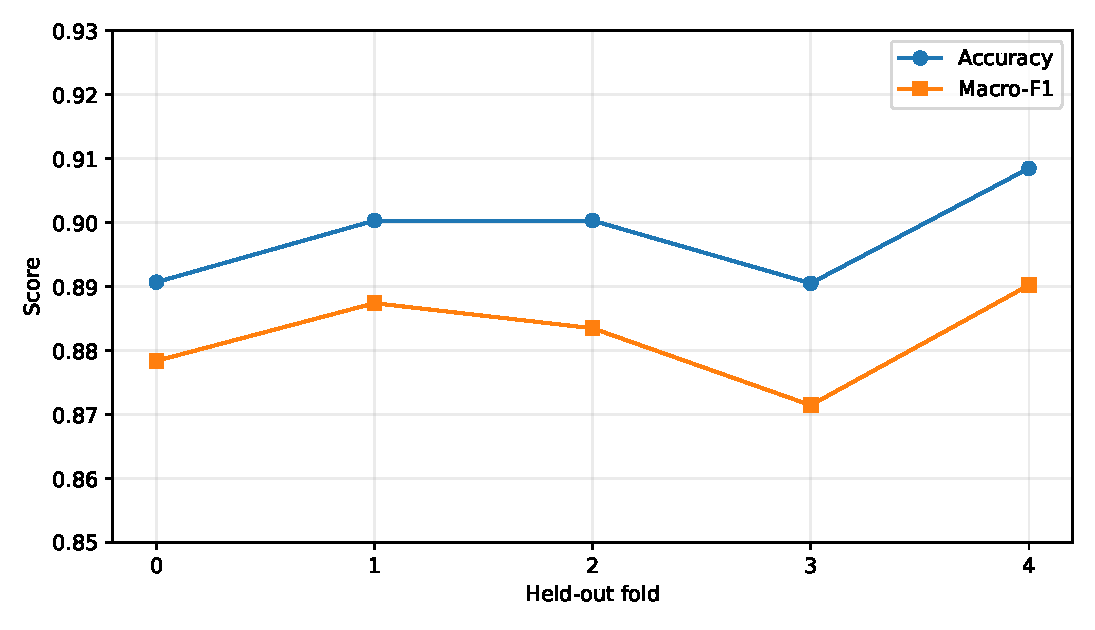
\includegraphics[width=0.98\columnwidth]{figures/fold_scores.pdf}
\caption{Five held-out fold accuracy and macro-F1 scores transcribed from independently checked Colab evaluation logs. These are different partitions, not independent random-seed repetitions.}\label{fig:foldscores}
\end{figure}

\begin{figure}[t]
\centering
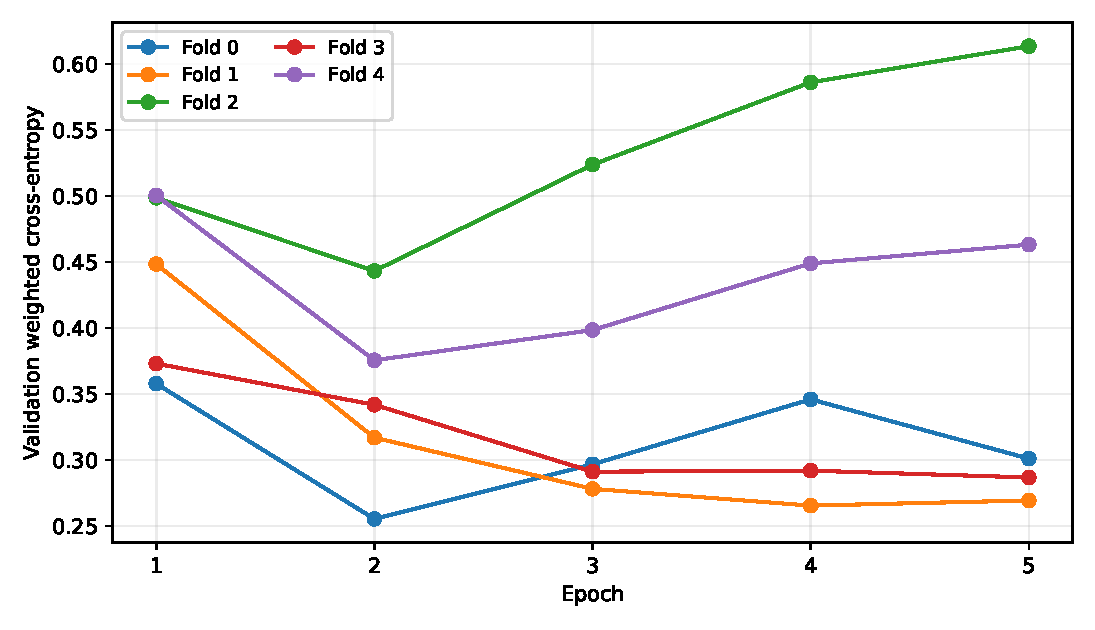
\includegraphics[width=0.98\columnwidth]{figures/validation_losses.pdf}
\caption{Validation weighted-cross-entropy by epoch, transcribed from genuine printed training logs (four decimal places). No smoothing or extrapolation is applied.}\label{fig:valloss}
\end{figure}

\subsection{Pooled out-of-fold predictions}
Across all 3,061 non-overlapping OOF assignments, 2,749 predictions were correct and 312 incorrect, giving pooled accuracy 0.898073 and pooled macro-F1 0.882170. The pooled confusion matrix in Table~\ref{tab:confusion} shows 77 true no-relationship sentences labeled correlation, the largest individual off-diagonal count. The conditional-causal category achieved 186 correct predictions out of 213 actual examples. The class-specific observations identify failure patterns but do not determine their causes.

\begin{table}[t]
\centering
\caption{Pooled OOF Confusion Matrix: Rows Actual, Columns Predicted}\label{tab:confusion}
\begin{tabular}{@{}lrrrr@{}}
\toprule
Actual & 0 & 1 & 2 & 3\\
\midrule
0 & 1206 & 48 & 25 & 77\\
1 & 38 & 426 & 13 & 17\\
2 & 17 & 6 & 186 & 4\\
3 & 48 & 15 & 4 & 931\\
\bottomrule
\end{tabular}
\end{table}

\subsection{Variation, loss trends, and possible mechanisms}
Fold accuracy ranged from 0.890523 to 0.908497, and fold macro-F1 from 0.871472 to 0.890226. These ranges summarize different data partitions, not independent restarts on identical partitions. Training loss declined across all five epochs of all five folds. In multiple folds validation loss increased after an earlier minimum, consistent with possible overfitting or increased confidence in erroneous predictions. Neither explanation is uniquely identified by these logs; differing fold composition and stochastic training also remain possible contributors.

\subsection{Computational cost and reproducibility evidence}
Fold 0 logged 283.5 elapsed seconds on the Tesla T4 for its measured experiment. Total observed runtime across all five folds was not supplied and remains [TO VERIFY]. The saved parameter checkpoint occupied 433,337,475 bytes per fold (approximately 2.17 GB for five checkpoints). Independent file-level audits validated all five prediction CSVs, their saved metrics, and row-to-label alignment. A strict checkpoint restore reproduced eight of eight inspected Fold 0 classifications, and all held-out predicted labels for Folds 1--4; the maximum absolute probability discrepancies for those four folds ranged from about $1.31\times10^{-6}$ to $5.25\times10^{-6}$.


\subsection{Class-Conditional Error Audit}
From the pooled OOF matrix, no-relationship statements were confused with correlation 77 times, while 48 correlational statements were incorrectly assigned no relationship. These asymmetries matter because a false positive for relationship language has different consequences from a false negative when interpreting a scientific claim. Class 2 (conditional causal) yielded 186 correct assignments among 213 gold items. At a dataset level, the corresponding recall is about 0.873; the model also produces false positive conditional labels on other categories. These patterns are derived exclusively from observed classifications and are not evidence of what the original authors intended in any individual sentence.

Class sizes are substantially unequal: 1,356 for no relationship, 494 for direct causality, 213 for conditional causality, and 998 for correlation. Overall accuracy is influenced disproportionately by the larger groups; macro-F1 weights all four class-specific F1 values equally. This choice of metric does not eliminate uncertainty from a small minority class, and no bootstrap intervals or independent reruns were performed.

\subsection{Loss Curves and Model Selection}
Figure~\ref{fig:valloss} reports the observed validation-loss trajectories across the fixed five-epoch training schedules. All folds showed a consistent decline in training loss. Fold 2 validation loss reached 0.4432 by epoch 2 and then rose to 0.6135 by epoch 5, while Fold 4 validation loss rose from 0.3755 at epoch 2 to 0.4631 at epoch 5. Such divergence is compatible with overfitting or confidence changes; it is not a test identifying a unique mechanism. The fifth-epoch model was retained even when an earlier epoch had better validation loss. Changing the stopping rule retroactively would create an unreported methodological adaptation.

\subsection{Limits of the Performance Comparison}
Figure~\ref{fig:foldscores} shows between-fold variation rather than independent-run uncertainty. The 0.001925 accuracy difference and 0.000797 macro-F1 difference from the rounded historical repository summary should not be described as statistically equivalent, superior or inferior in the absence of matched folds and a prespecified comparison. A majority-class rule would attain 1,356/3,061 accuracy on the same class distribution, but no such method was independently trained and assessed under the frozen protocol here; it is a descriptive class-frequency calculation, not a second executed baseline. There is likewise no evidence that a new algorithm has improved performance.

\section{Limitations}\label{sec:limits}
This work establishes an internally audited modern result, not exact historical execution. In particular, the historical and contemporary outer-fold sizes differ, the internal validation RNG pathway differs, the historical BioBERT archive has not been verified tensor by tensor against the pinned contemporary checkpoint, and the optimizer is a source-guided implementation rather than the original package. Model weights were initialized and trained once per partition; no repeated-seed variability estimate is available.

The full-corpus class weights expose held-out label frequencies to training. The seven duplicate sentence pairs include at least some cross-partition text overlap, so row-index separation does not ensure complete text-level independence. Possible character-encoding artifacts and the relatively small, imbalanced PubMed corpus further limit interpretation. No external-domain, sentence-pair editing, human semantic-preservation, causal-direction, or certainty calibration experiment was conducted. Consequently, accuracy and macro-F1 cannot be interpreted as measures of causal-meaning preservation after LLM editing. Dataset-specific reuse rights, annotation reliability and exact overlap counts under archived folds remain [TO VERIFY].


\section{Independent Verification Procedure}\label{sec:verification}
The actual verification campaign was sequential and preserved an audit trail of each module's successful console output. First, the original implementation and historical optimizer source were inspected rather than inferred from a generic BERT fine-tuning recipe. The historical optimizer differs from PyTorch AdamW in its absence of standard bias correction, per-parameter rather than global gradient clipping, parameter-group decay handling, and scheduling based on the current step before incrementing it. A deterministic two-parameter, three-step numerical check compared two source-derived update calculations and returned zero maximum parameter difference for those inputs. The test was then extended to a real BioBERT encoder plus classification head; its first scheduled step left weights unchanged, and the following step produced nonzero, finite changes in both head and encoder. This is evidence about tested behavior only, not a guarantee of algorithmic equivalence for all historical software paths.

Second, before any cross-validation model was trained, five outer-fold manifests were saved. Each manifest contained the fit, internal validation and test indices and a stated RNG choice. Per-fold assertions checked non-overlap among partitions and full corpus coverage by row ID. After all five runs, a global aggregation verified exactly one held-out prediction per original row. Because multiple sentence strings can be equal, ID-level coverage alone cannot establish independence of exact text content. The initial data audit located seven duplicate pairs and one conflicting-label pair; these were preserved for comparability and disclosed as a threat to validity.

Third, independently of the trained model, the saved CSV files were read back and evaluated. For each fold, the audits verified the number and uniqueness of original row identifiers, the true labels at those source rows, the four finite probability values per item, probability normalization, agreement between argmax and saved predicted labels, and equality between recomputed and stored accuracy and macro-F1. The final aggregation independently checked the fivefold arithmetic averages and sample standard deviations. The pooled confusion matrix was recalculated from the saved non-overlapping held-out records. This is the main evidence for the numerical validity of the results; consistency between saved artifacts and code output is necessary but not a demonstration of external generalization.

Finally, all five trained checkpoints passed strict weight-loading checks. For Fold 0, eight held-out examples were re-evaluated with restored parameters, with maximum probability difference approximately $6.05\times10^{-9}$. For Folds 1--4, the complete held-out partitions of 612 examples each were re-evaluated, and no class-label mismatches were found. The largest maximum probability difference across those four complete-fold tests was about $5.25\times10^{-6}$. Independent checkpoint restoration ensures that the saved parameters are usable and consistent with the saved inference outputs within the tested tolerance; it does not validate the original historical pretrained model archive.

\section{Threats to Validity and Reporting Integrity}\label{sec:threats}
\emph{Internal validity:} The baseline's use of global class frequencies leaks a small amount of label-distribution information from held-out partitions into the class-weighted objective. As this feature was verified in the historical source, it was retained to preserve the specific reproduced protocol; it must not be described as an ideal leakage-free model-selection or benchmark design. A separate controlled run with training-only class weights is needed to determine whether the observed performance is sensitive to this design choice. Without that run, neither the magnitude nor the sign of an effect can be stated.

\emph{Construct validity:} The corpus provides categorical judgments about the wording of individual conclusion sentences. It does not supply a causal graph, actual intervention outcomes or human annotation of two alternate wordings for the same underlying result. A classifier that returns the same class before and after editing can still miss changed causal direction, qualifiers, entity references or certainty. Conversely, changed labels are not invariably a meaningful semantic change. Therefore neither accuracy nor macro-F1 is a direct metric of causal preservation in LLM editing.

\emph{Statistical validity:} Each cross-validation fold was trained with one configured seed, but different folds expose different training and test examples. The sample standard deviation across folds captures variation in this observed cross-validation procedure, not the distribution across repeated stochastic model restarts or a confidence interval for a new publication domain. Historical means are rounded and obtained with different folds. No statistical significance or equivalence test was carried out, and conclusions should not treat small differences as evidence for improved or degraded algorithms.

\emph{External validity:} The evaluation uses one PubMed-derived corpus with label imbalance. It does not address different research fields, longer document-level contexts, languages beyond the existing resource or contemporary human/LLM editing workflows. The model may be useful as a baseline for future paired-editing investigation, but that utility remains a conjecture until the experiment is executed. Also, imperfect encoding in some strings, annotation ambiguity and duplicate content may introduce error mechanisms not separable from model weaknesses using only the aggregated confusion matrix.

\emph{Artifact and attribution integrity:} The verification record was supplied as authentic Colab logs and referenced local result files, but the complete raw notebook, per-row prediction CSVs, frozen manifests, exact package freeze and fine-tuned checkpoints are not bundled in the current submission kit. A stand-alone verification script is provided for later execution once those original artifacts are exported. Claims about an independent clean-room rerun or full public reproducibility must remain conditional on this transfer. The original classification architecture, BioBERT pretraining and historical code are credited to their respective authors; the contribution claimed here is source-guided verification and reporting, not invention of the baseline classifier.

\section{Planned Extension (Not Evaluated)}\label{sec:future}
The motivation for the follow-up study arises from the supplied literature review's proposed editing-preservation benchmark. A future corpus would contain an original scientific conclusion sentence, a controlled edit, the study-design context when available, and independent annotator judgments about whether the edit preserves claim type, hedge strength, scope and causal direction. At least two categories should be deliberately present: genuinely meaning-preserving paraphrases and changes such as associational-to-causal inflation or removal of uncertainty language. The number of items, sampling frame, annotator identities, annotation rubric, inter-annotator agreement and source licensing must be established before data collection. **No such dataset or experiment is included in the present reported results.**

A controlled study could then compare (i) a frozen four-class BioBERT label-change detector, (ii) a preregistered simpler lexical or rule-based control, and (iii) independently agreed human preservation labels as the evaluation target. Each comparator should receive exactly the same paired inputs, access only to its permitted context, and use a common held-out split. This design would avoid conflating a method comparison with differences in evaluation partitions. If the study instead tests training-only class weighting, the revised weighting must be assessed as a distinct sensitivity condition with unchanged outer test indices, rather than replacing the published-style historical baseline retrospectively.

The principal quantitative outcomes should reflect the newly defined question: macro-F1 for human-annotated preservation versus change, false alarms on accepted paraphrases, missed causal inflation, and error rates by editing operation. Class-label agreement alone is only a proxy for the target; a direct human label is required to test the preservation question. Annotation uncertainty should be reported, and uncertain or disputed items should be handled by a policy defined before model selection. The protocol should forbid editing prompts, thresholds or classifier weights from being selected using the final held-out pair set. Confidence intervals or repeated seeds should be used only when the sampling and evaluation assumptions permit meaningful inference.

This extension is proposed as a next-stage experimental plan, **not a demonstrated contribution or performance improvement**. To meet the assignment's experimental-comparison gate, the additional experiment must actually be executed, documented with genuine logs, audited for input alignment and reported irrespective of whether the frozen classifier performs well. Negative results would remain informative: a simple four-class classifier may be insensitive to strength and direction changes within the same label, underscoring the difference between broad linguistic classification and claim-level semantic fidelity.

\section{Conclusion}\label{sec:conclusion}
A source-guided modern implementation of the four-class BioBERT causal-language classifier achieved mean five-fold accuracy 0.8981 and mean macro-F1 0.8822 on 3,061 PubMed sentences, close to published rounded reference values of 0.900 and 0.883. Complete OOF row coverage and independent prediction-metric consistency were verified, and each fold's saved checkpoint passed a restoration test of the specified scope. Methodological differences and possible benchmark leakage prevent a claim of exact historical replication or leakage-free generalization. A separately annotated source--edited corpus is needed before causal-meaning preservation under LLM-assisted editing can be assessed.

% BibTeX metadata also provided in references.bib. A direct bibliography
% is used in this offline build because the bibtex executable is absent.
\begin{thebibliography}{2}
\bibitem{yu2019detecting} B. Yu, Y. Li, and J. Wang, ``Detecting Causal Language Use in Science Findings,'' in \emph{Proc. EMNLP-IJCNLP}, 2019, pp. 4664--4674, doi: \href{https://doi.org/10.18653/v1/D19-1473}{10.18653/v1/D19-1473}.
\bibitem{lee2020biobert} J. Lee \emph{et al.}, ``BioBERT: a pre-trained biomedical language representation model for biomedical text mining,'' \emph{Bioinformatics}, vol. 36, no. 4, pp. 1234--1240, 2020, doi: \href{https://doi.org/10.1093/bioinformatics/btz682}{10.1093/bioinformatics/btz682}.
\end{thebibliography}
\end{document}
